\documentclass[11pt,paper=a4,answers]{exam}
\usepackage{graphicx,lastpage}
\usepackage{upgreek}
\usepackage{censor}
\usepackage{gensymb}
\usepackage{amsmath}
\usepackage{multicol}
\usepackage{enumitem}
 \usepackage{pgfplots}
\pgfplotsset{compat=1.18}
\usepackage{tasks}
\usepackage{adjustbox}
\usepackage{xcolor}
\usepackage{tfrupee}
\setlength{\voffset}{0.25in}
\usepackage{tabularx}
\newcolumntype{Y}{>{\centering\arraybackslash}X}
%==============================================================
% Customise Non-Essential Packages Below
% =============================================================
\usepackage[most]{tcolorbox}
\usepackage{eso-pic}
\usepackage{tikz}
\AddToShipoutPictureBG{%
\begin{tikzpicture}[remember picture,overlay]
\foreach \x in {-8,-4,0,4,8,12,16,20}
\foreach \y in {-8,-4,0,4,8,12,16,20} {
\node[opacity=0.05,rotate=45,anchor=center] at ([xshift=\x cm,yshift=\y cm]current page.center) {%
\begin{minipage}{2cm}
\centering
\includegraphics[width=2cm]{images/logo_black.png}\\
\small preppeo.com
\end{minipage}%
};
}
\end{tikzpicture}%
}
\printanswers

%==============================================================
% Customise Non-Essential Packages Above
% =============================================================
\definecolor{svgray}{rgb}{0.90, 0.90, 0.90}
\graphicspath{{images/}}

\usepackage[normalem]{ulem}
\renewcommand\ULthickness{1pt}   %%---> For changing thickness of underline
\setlength\ULdepth{3.5ex}%\maxdimen ---> For changing depth of underline
\renewcommand{\baselinestretch}{1}
\chead{
\includegraphics[scale=0.1,height=2cm ]{logo.png}
}
\pagestyle{empty}

\pagestyle{headandfoot}
\headrule
\cfoot{W: https://preppeo.com; M: +91-8130711689}

\begin{document}
%==============================================================
% Customise Question paper details below this
% =============================================================
\begin{center}
    \centering
    \renewcommand{\arraystretch}{1.5}
    \begin{tabularx}{\textwidth}{YYY}
    & \normalsize\bf{{\Large{{Quantitative Reasoning}}}} & \\
    By Preppeo & \normalsize\bf{MOCK } & GRE\\
    \normalsize{\textbf{Questions:} 15 (Section 2 : 15} & \normalsize{\textbf{Marks:} 27 } & \normalsize{\textbf{Time:}  minutes } \\
    \end{tabularx}
\end{center}
\par\noindent\rule{\textwidth}{1pt}
% =============================================================
% Customise Question paper details above this
% =============================================================

\begin{questions}
\pointsinrightmargin
\pointsdroppedatright
\marksnotpoints
\pointpoints{mark}{marks}
\pointformat{\boldmath\themarginpoints}
\bracketedpoints

% =============================================================
% Question Begin
% =============================================================
\section*{Section 2 - Mock 4 Set 1 (Medium)}

% --- QUANTITY COMPARISON (5 QUESTIONS) ---

%Q: 1
\question
$m, n, p, \text{ and } q$ are integers such that $m > n$ and $p > q$.
\vspace{5pt}
\textbf{Quantity A: } $m + p$ \\
\vspace{5pt}
\textbf{Quantity B: } $n + q$

\begin{tasks}(1)
\task[A)] Quantity A is greater
\task[B)] Quantity B is greater
\task[C)] The two quantities are equal
\task[D)] The relationship cannot be determined
\end{tasks}

\begin{solution}
This question tests the fundamental properties of inequalities.
\vspace{5pt}
\begin{center}
We are given two inequalities: $m > n$ and $p > q$.
\vspace{5pt}
In algebra, if you add the larger sides of two inequalities, the sum is definitively larger than the sum of the smaller sides.
\vspace{5pt}
$m + p > n + q$
\end{center}
\vspace{5pt}
Therefore, Quantity A is always greater than Quantity B.

Answer: \colorbox{yellow!100}{A}
\end{solution}

\vspace{1cm}

%Q: 2
\question
A dataset of test scores is normally distributed with a mean of 550 and a standard deviation of 40.
\vspace{5pt}
\textbf{Quantity A: } The percentile of a score of 590 \\
\vspace{5pt}
\textbf{Quantity B: } 84

\begin{tasks}(1)
\task[A)] Quantity A is greater
\task[B)] Quantity B is greater
\task[C)] The two quantities are equal
\task[D)] The relationship cannot be determined
\end{tasks}

\begin{solution}
First, determine how many standard deviations the score is from the mean.
\vspace{5pt}
\begin{center}
$Z = \dfrac{\text{Score} - \text{Mean}}{\text{Standard Deviation}} = \dfrac{590 - 550}{40} = \dfrac{40}{40} = 1$
\end{center}
\vspace{5pt}
In a normal distribution, a score that is exactly 1 standard deviation above the mean is at the 84th percentile.
\vspace{5pt}
\begin{center}
Percentile $= 50\% (\text{below mean}) + 34\% (\text{between mean and } +1\sigma) = 84\%$
\end{center}
\vspace{5pt}
Quantity A is 84 and Quantity B is 84.

Answer: \colorbox{yellow!100}{C}
\end{solution}

\vspace{1cm}

%Q: 3
\question
\begin{center}
\begin{tikzpicture}[scale=1.2]
    \draw[thick] (0,0) coordinate (A) -- (3,0) coordinate (C) -- (1,2) coordinate (B) -- cycle;
    \draw[thick, dashed] (0.5, 1) -- (2, 1);
    \node[left] at (A) {$A$};
    \node[right] at (C) {$C$};
    \node[above] at (B) {$B$};
    \node at (1.5, 1) [above] {$k$};
    \node at (1.5, 0) [below] {$B$};
\end{tikzpicture}
\end{center}
In the triangle above, the dashed line segment $k$ is parallel to the base $B$ and bisects the other two sides.
\vspace{5pt}
\textbf{Quantity A: } The ratio of $k$ to $B$ \\
\vspace{5pt}
\textbf{Quantity B: } 0.5

\begin{tasks}(1)
\task[A)] Quantity A is greater
\task[B)] Quantity B is greater
\task[C)] The two quantities are equal
\task[D)] The relationship cannot be determined
\end{tasks}

\begin{solution}
According to the Triangle Midsegment Theorem, a segment connecting the midpoints of two sides of a triangle is parallel to the third side and is exactly half its length.
\vspace{5pt}
\begin{center}
$k = \dfrac{1}{2}B \implies \dfrac{k}{B} = 0.5$
\end{center}
\vspace{5pt}
Quantity A is 0.5 and Quantity B is 0.5.

Answer: \colorbox{yellow!100}{C}
\end{solution}

\vspace{1cm}

%Q: 4
\question
$x$ is a positive integer such that $4^x$ is a factor of $20!$.
\vspace{5pt}
\textbf{Quantity A: } The greatest possible value for $x$ \\
\vspace{5pt}
\textbf{Quantity B: } 9

\begin{tasks}(1)
\task[A)] Quantity A is greater
\task[B)] Quantity B is greater
\task[C)] The two quantities are equal
\task[D)] The relationship cannot be determined
\end{tasks}

\begin{solution}
First, find the highest power of prime 2 that divides $20!$ using Legendre's Formula:
\vspace{5pt}
\begin{center}
$\lfloor 20/2 \rfloor + \lfloor 20/4 \rfloor + \lfloor 20/8 \rfloor + \lfloor 20/16 \rfloor = 10 + 5 + 2 + 1 = 18$
\end{center}
\vspace{5pt}
So, $2^{18}$ divides $20!$. We need to find the power of $4$ (which is $2^2$).
\vspace{5pt}
\begin{center}
$4^x = (2^2)^x = 2^{2x}$
\vspace{5pt}
$2x = 18 \implies x = 9$
\end{center}
\vspace{5pt}
Quantity A is 9 and Quantity B is 9.

Answer: \colorbox{yellow!100}{C}
\end{solution}

\vspace{1cm}

%Q: 5
\question
\[ rs = \sqrt{3} \]
\vspace{5pt}
\textbf{Quantity A: } $\dfrac{rs}{3}$ \\
\vspace{5pt}
\textbf{Quantity B: } $\dfrac{2}{3\sqrt{2}}$

\begin{tasks}(1)
\task[A)] Quantity A is greater
\task[B)] Quantity B is greater
\task[C)] The two quantities are equal
\task[D)] The relationship cannot be determined
\end{tasks}

\begin{solution}
Simplify both quantities to compare their numerical values.
\vspace{5pt}
\begin{center}
Quantity A: $\dfrac{\sqrt{3}}{3} \approx \dfrac{1.732}{3} \approx 0.577$
\vspace{5pt}
Quantity B: $\dfrac{2}{3\sqrt{2}} = \dfrac{2}{3(1.414)} = \dfrac{2}{4.242} \approx 0.471$
\end{center}
\vspace{5pt}
Since 0.577 is greater than 0.471, Quantity A is greater.

Answer: \colorbox{yellow!100}{A}
\end{solution}

\vspace{1cm}

% --- MCQ SINGLE CHOICE (5 QUESTIONS) ---

%Q: 6
\question
A jewelry store sells silver rings for \$80 and gold rings for \$240. If the average price of 50 rings sold was \$144, how many gold rings were sold?

\begin{tasks}(1)
\task[A)] 15 \task[B)] 20 \task[C)] 25 \task[D)] 30 \task[E)] 35
\end{tasks}

\begin{solution}
Let $g$ be the number of gold rings and $s$ be the number of silver rings.
\vspace{5pt}
\begin{center}
$g + s = 50 \implies s = 50 - g$
\vspace{5pt}
$240g + 80s = 50 \times 144 = 7200$
\vspace{5pt}
$240g + 80(50 - g) = 7200$
\vspace{5pt}
$240g + 4000 - 80g = 7200$
\vspace{5pt}
$160g = 3200 \implies g = 20$
\end{center}

Answer: \colorbox{yellow!100}{B}
\end{solution}

\vspace{1cm}

%Q: 7
\question
What is the greatest prime factor of $3^{20} - 3^{18}$?

\begin{tasks}(1)
\task[A)] 2 \task[B)] 3 \task[C)] 5 \task[D)] 7 \task[E)] 11
\end{tasks}

\begin{solution}
Factor the expression to identify its prime components.
\vspace{5pt}
\begin{center}
$3^{20} - 3^{18} = 3^{18}(3^2 - 1)$
\vspace{5pt}
$3^{18}(9 - 1) = 3^{18}(8) = 3^{18} \times 2^3$
\end{center}
\vspace{5pt}
The prime factors are 2 and 3. The greatest prime factor is 3.

Answer: \colorbox{yellow!100}{B}
\end{solution}

\vspace{1cm}

%Q: 8
\question
\begin{center}
\begin{tikzpicture}
\begin{axis}[
    axis lines=middle,
    xmin=-4, xmax=4,
    ymin=-5, ymax=5,
    grid=major,
    width=8cm, height=6cm
]
\addplot[domain=-2.2:2.2, samples=100, thick, blue] {-x^2 + 1};
\end{axis}
\end{tikzpicture}
\end{center}
Which of the following is the equation of the parabola shown above?

\begin{tasks}(1)
\task[A)] $y = x^2 + 1$ \task[B)] $y = -x^2 + 1$ \task[C)] $y = -x^2 - 1$ \task[D)] $y = -(x-1)^2$ \task[E)] $y = x^2 - 1$
\end{tasks}

\begin{solution}
Analyze the graph's properties.
\vspace{5pt}
\begin{center}
The parabola opens downward, so the $x^2$ coefficient must be negative.
\vspace{5pt}
The vertex (y-intercept) is at $(0, 1)$.
\vspace{5pt}
Testing $x=0$: $y = -(0)^2 + 1 = 1$. (Matches graph)
\end{center}

Answer: \colorbox{yellow!100}{B}
\end{solution}

\vspace{1cm}

%Q: 9
\question
If $g$ is an integer and $x$ is a prime number, which of the following \textbf{must} be an integer?

\begin{tasks}(1)
\task[A)] $\dfrac{g^2x + 7gx}{x}$ \task[B)] $g^2 - \dfrac{x}{3}$ \task[C)] $\dfrac{x}{g}$ \task[D)] $\dfrac{g}{x}$ \task[E)] $\sqrt{gx}$
\end{tasks}

\begin{solution}
Evaluate the algebraic properties of each expression.
\vspace{5pt}
\begin{center}
$\dfrac{x(g^2 + 7g)}{x} = g^2 + 7g$
\end{center}
\vspace{5pt}
Since $g$ is an integer, $g^2 + 7g$ will always result in an integer value.

Answer: \colorbox{yellow!100}{A}
\end{solution}

\vspace{1cm}

%Q: 10
\question
A cylindrical tank has a diameter of 6 meters and a height of 10 meters. If it is 60\% full, what is the volume of water in cubic meters?

\begin{tasks}(1)
\task[A)] $36\pi$ \task[B)] $54\pi$ \task[C)] $60\pi$ \task[D)] $90\pi$ \task[E)] $120\pi$
\end{tasks}

\begin{solution}
\begin{center}
Radius $r = 6 / 2 = 3$
\vspace{5pt}
Full Volume $V = \pi r^2 h = \pi \times 3^2 \times 10 = 90\pi$
\vspace{5pt}
60\% Volume $= 0.60 \times 90\pi = 54\pi$
\end{center}

Answer: \colorbox{yellow!100}{B}
\end{solution}

\vspace{1cm}

% --- MCQ MULTIPLE CHOICE (1 QUESTION) ---

%Q: 11
\question
If $a, b, \text{ and } c$ are consecutive integers such that $a < b < c$, which of the following \textbf{must} be even?
Indicate \textbf{all} such expressions.

\begin{tasks}(1)
\task[A)] $abc$
\task[B)] $a + b + c$
\task[C)] $(a+b)(b+c)$
\end{tasks}

\begin{solution}
\begin{center}
Statement A: In any three consecutive integers, at least one is even. Their product must be even. (True)
\vspace{5pt}
Statement B: If $a=2, b=3, c=4$, sum is 9. (False)
\vspace{5pt}
Statement C: If $a=1, b=2, c=3$, then $(1+2)(2+3) = 3 \times 5 = 15$. (False)
\end{center}

Answer: \colorbox{yellow!100}{A}
\end{solution}

\vspace{1cm}

% --- INPUT QUESTION (1 QUESTION) ---

%Q: 12
\question
What is the units digit of $2^{43} + 3^{43}$?

\begin{solution}
\begin{center}
$2^x$ cycle: 2, 4, 8, 6. $43 / 4 \to \text{rem } 3 \to 8$.
\vspace{5pt}
$3^x$ cycle: 3, 9, 7, 1. $43 / 4 \to \text{rem } 3 \to 7$.
\vspace{5pt}
Sum of digits: $8 + 7 = 15 \to 5$.
\end{center}

Answer: \colorbox{yellow!100}{5}
\end{solution}

\vspace{1cm}

% --- DATA INTERPRETATION (3 QUESTIONS) ---
\textbf{Questions 13-15 refer to the following graph.}

\begin{center}
\begin{tikzpicture}
\begin{axis}[
    ybar,
    symbolic x coords={2021, 2022, 2023, 2024},
    xtick=data,
    ylabel={Profit (\$ Millions)},
    ymin=0, ymax=60,
    grid=major,
    width=8cm, height=6cm
]
\addplot coordinates {(2021,20) (2022,35) (2023,50) (2024,45)};
\end{axis}
\end{tikzpicture}
\end{center}

%Q: 13
\question
What was the average annual profit over the four-year period?

\begin{tasks}(1)
\task[A)] \$35.0M \task[B)] \$37.5M \task[C)] \$40.0M \task[D)] \$42.5M \task[E)] \$45.0M
\end{tasks}

\begin{solution}
\begin{center}
Sum $= 20 + 35 + 50 + 45 = 150$
\vspace{5pt}
Average $= 150 / 4 = 37.5$
\end{center}

Answer: \colorbox{yellow!100}{B}
\end{solution}

\vspace{1cm}

%Q: 14
\question
What was the percentage increase in profit from 2021 to 2023?

\begin{tasks}(1)
\task[A)] 50 percent \task[B)] 75 percent \task[C)] 100 percent \task[D)] 150 percent \task[E)] 250%
\end{tasks}

\begin{solution}
\begin{center}
Increase $= 50 - 20 = 30$
\vspace{5pt}
Percentage Increase $= (30 / 20) \times 100 = 150\%$
\end{center}

Answer: \colorbox{yellow!100}{D}
\end{solution}

\vspace{1cm}

%Q: 15
\question
Based on the chart, which of the following statements are true?
Indicate \textbf{all} such statements.

\begin{tasks}(1)
\task[A)] The median profit was 40.0M.
\task[B)] Profit increased in every year shown.
\task[C)] The total profit for the first two years was less than the profit in 2023.
\end{tasks}

\begin{solution}
\begin{center}
Statement A: Ordered set $\{20, 35, 45, 50\}$. Median $= (35+45)/2 = 40$. (True)
\vspace{5pt}
Statement B: Profit decreased between 2023 and 2024. (False)
\vspace{5pt}
Statement C: $20 + 35 = 55$. 55 is NOT less than 50. (False)
\end{center}

Answer: \colorbox{yellow!100}{A}
\end{solution}

% =============================================================
% Question End
% =============================================================

\end{questions}
\begin{center}
\rule{.5\textwidth}{1pt}
\end{center}
\end{document}
